\subsection{Results}
\label{sec:results}

We decided to compare the results for three different models. Below you can find two tables - one of them is based on the results which were achieved using all the available data sources we have (which includes the questionnaire) \textit{[ref: table\ref{table:1}]}  while the other uses only the data that can be gathered using GraphQL request to GitHub API and the Mega Linter with parsing scripts \textit{[ref: table\ref{table:2}]}. In the second case, we used \code{AvgCommitTime}, \code{DupLinesPercent} and \code{LinesPerFile} attributes. Below the tables, we present the correlation matrix of individual features \textit{[ref: figure\ref{fig:correlation-matrix}]}. 

\begin{table}[h!]
\centering
\begin{tabular}{ | m{5em} | m{5em}| m{5em} | m{5em}| m{5em} | m{5em}| } 
\hline
 Algorithm & \textbf{MMCE} & \textbf{MCC} & \textbf{F1} & \textbf{ACC} & \textbf{Kappa}\\ 
 \hline
 \textbf{Random Forest} & 0.329 & 0.245 & 0.410 & 0.671 & 0.219 \\ 
\hline
 \textbf{SVM} & 0.315 & 0.356 & 0.422 & 0.685 & 0.311 \\ 
\hline
 \textbf{KNN} & 0.388 & 0.224 & 0.431 & 0.611 & 0.184\\ 
\hline
\end{tabular}
\caption{Measures scores for each classifiers (all features)}
\label{table:1}
\end{table}

\begin{table}[h!]
\centering
\begin{tabular}{ | m{5em} | m{5em}| m{5em} | m{5em}| m{5em} | m{5em}| } 
\hline
 Algorithm & \textbf{MMCE} & \textbf{MCC} & \textbf{F1} & \textbf{ACC} & \textbf{Kappa}\\ 
 \hline
 \textbf{Random Forest} & 0.360 & 0.299 & 0.451 & 0.639 & 0.245 \\ 
\hline
 \textbf{SVM} & 0.319 & 0.314 & 0.451 & 0.680 & 0.280 \\ 
\hline
 \textbf{KNN} & 0.367 & 0.237 & 0.484 & 0.632 & 0.209\\ 
\hline
\end{tabular}
\caption{Measures scores for each classifiers (\emph{GitHub API} and \emph{Mega Linter} features)}
\label{table:2}
\end{table}

\begin{figure}[htp]
\centering
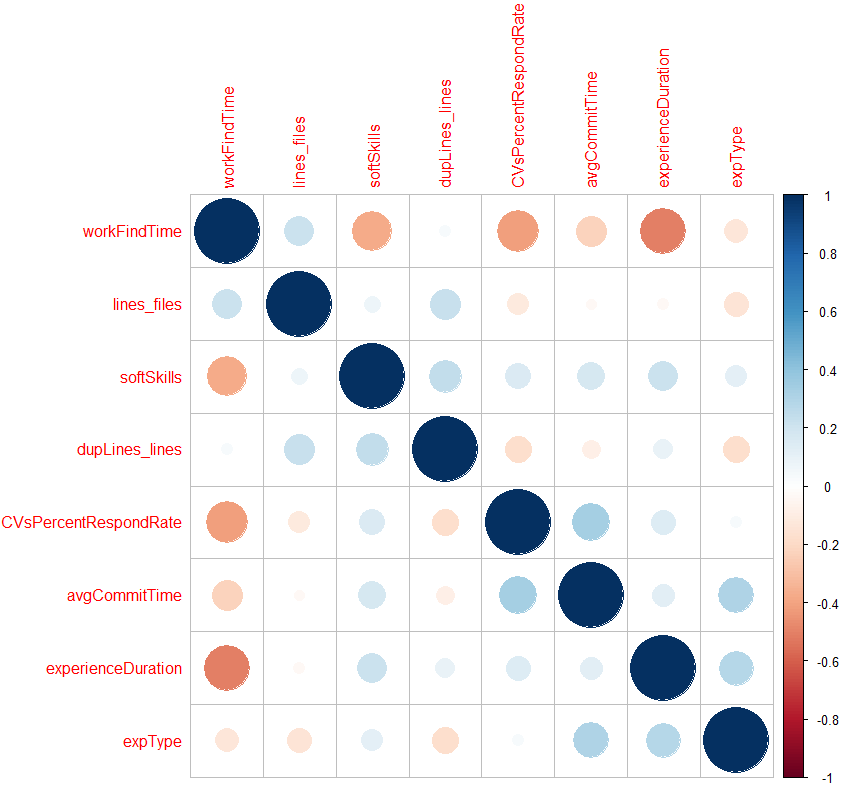
\includegraphics[width=\linewidth]{r_plot_corrrelation.png}
\caption{Correlation Matrix}
\label{fig:correlation-matrix}
\end{figure}
